
%Dạng 50
\setcounter{ex}{0}
\section{Tính đơn điệu của hàm số liên kết}
\subsection{Kiến thức cần nhớ.}
\begin{khung}
	\subsubsection{Định nghĩa}
	Giả sử $\mathcal{K}$ là một khoảng, đoạn hoặc nửa khoảng và $y=f(x)$ là một hàm số xác định trên $\mathcal{K}$. Ta nói
	\begin{itemize}
		\item Hàm số $y=f(x)$ được gọi là \emph{\textbf{đồng biến}} (tăng) trên $\mathcal{K}$ nếu
		\[\forall x_1,x_2\in \mathcal{K}, x_1<x_2 \Rightarrow f(x_1)<f(x_2).\]
		\item Hàm số $y=f(x)$ được gọi là \emph{\textbf{nghịch biến}} (giảm) trên $\mathcal{K}$ nếu
		\[\forall x_1,x_2\in \mathcal{K}, x_1<x_2 \Rightarrow f(x_1)>f(x_2).\]
	\end{itemize}
	Hàm số đồng biến hoặc nghịch biến trên $\mathcal{K}$ gọi chung là \emph{\textbf{đơn điệu}} trên $\mathcal{K}$.
	
	\subsubsection{Tính chất}
	\begin{enumerate}
		\item Nếu hàm số $f(x)$ và $g(x)$ cùng đồng biến (nghịch biến) trên $\mathcal{K}$ thì hàm số $f(x)+g(x)$ cũng đồng biến (nghịch biến) trên $\mathcal{K}$.\\
		Tính chất này có thể không đúng đối với hiệu $f(x)-g(x)$.
		\item Nếu hàm số $f(x)$ và $g(x)$ là các hàm số dương và cùng đồng biến (nghịch biến) trên $\mathcal{K}$ thì hàm số $f(x)\cdot g(x)$ cũng đồng biến (nghịch biến) trên $\mathcal{K}$.\\
		Tính chất này có thể không đúng khi các hàm số $f(x)$, $g(x)$ không là các hàm số dương trên $\mathcal{K}$.
		\item Cho hàm số $u=u(x)$ xác định với mọi $x\in (a;b)$ và $u(x)\in (c;d)$. Hàm số $f\left(u(x)\right)$ cũng xác định với $x\in (a;b)$. Ta có nhận xét sau:
		\begin{enumerate}[i)]
			\item Giả sử hàm số $u=u(x)$ đồng biến với mọi $x\in (a;b)$. Khi đó , hàm số $f\left(u(x)\right)$ đồng biến trên $ (a;b)$ khi và chỉ khi $f(u)$ đồng biến trên $(c;d)$.
			\item Giả sử hàm số $u=u(x)$ nghịch biến với mọi $x\in (a;b)$. Khi đó, hàm số $f\left(u(x)\right)$ nghịch biến $(a;b)$ khi và chỉ khi $f(u)$ nghịch biến $(c;d)$.
		\end{enumerate}
	\end{enumerate}
	
	
	\subsubsection{Định lí 1}
	Giả sử hàm số $f$ có đạo hàm trên khoảng $\mathcal{K}$. Khi đó
	\begin{itemize}
		\item Nếu $f'(x)> 0, \forall x\in \mathcal{K}$ thì hàm số $f$ đồng biến trên $\mathcal{K}$.
		\item Nếu $f'(x)< 0, \forall x\in \mathcal{K}$ thì hàm số $f$ nghịch biến trên $\mathcal{K}$.
		\item Nếu $f'(x)= 0, \forall x\in \mathcal{K}$ thì hàm số $f$ không đổi trên $\mathcal{K}$.
	\end{itemize}
	\begin{note}
		Khoảng $\mathcal{K}$ trong định lí trên ta có thể thay thế bởi đoạn hoặc nửa khoảng. Khi đó phải có thêm giả thiết ``Hàm số liên tục trên đoạn hoặc nửa khoảng đó''. Chẳng hạn, nếu hàm số $f$ liên tục trên đoạn $[a;b]$ và $f'(x)>0, \forall x\in (a;b)$ thì hàm số $f$ đồng biến trên đoạn $[a;b]$. Ta thường biểu diễn qua bảng biến thiên như sau:
		\begin{center}
			\begin{tikzpicture}
				\tkzTabInit[lgt=1.5,espcl=5,deltacl=0.6]
				{$x$/0.6, $f'(x)$/0.6, $f(x)$/2}
				{$a$, $b$}
				\tkzTabLine{,+,}
				\tkzTabVar{-/$f(a)$, +/$f(b)$}
			\end{tikzpicture}
		\end{center}
	\end{note}
	
	\subsubsection{Định lí 2}
	Giả sử hàm số $f$ có đạo hàm trên khoảng $\mathcal{K}$. Khi đó
	\begin{itemize}
		\item Nếu $f'(x)\geq 0, \forall x\in \mathcal{K}$ và $f'(x)=0$ chỉ tại hữu hạn điểm thuộc $\mathcal{K}$ thì hàm số $f$ đồng biến trên $\mathcal{K}$.
		\item Nếu $f'(x)\leq 0, \forall x\in \mathcal{K}$ và $f'(x)=0$ chỉ tại hữu hạn điểm thuộc $\mathcal{K}$ thì hàm số $f$ nghịch biến trên $\mathcal{K}$.
	\end{itemize}
	\emph{\textbf{Quy tắc xét tính đơn điệu của hàm số}}\\
	Giả sử hàm số $f$ có đạo hàm trên $\mathcal{K}$.\\
	Hàm số $y=\left|f(x) \right|$ đồng biến trên tập $\mathrm{K}$ khi và chỉ khi $f^2(x)$ đồng biến trên $\mathrm{K} \Leftrightarrow f'(x) \cdot f(x) \geq 0$ với $\forall x \in \mathrm{K}.$
\end{khung}

%======================================
\subsection{Bài tập mẫu}
\Opensolutionfile{ans}[ans/ANS-DANG-50]
\begin{khung}
	\begin{vd}[Đề minh họa BGD 2022-2023]%[2D1G1-3]
		Có bao nhiêu giá trị nguyên của tham số $a\in(-10;+\infty)$ để hàm số\\ $y=\left|x^3+(a+2) x+9-a^2\right|$ đồng biến trên khoảng $(0;1)$?
		\choice
		{$12$}
		{\True $11$}
		{$6$}
		{$5$}
		\loigiai{
			Xét $f(x)=x^3+(a+2) x+9-a^2 \Rightarrow f'(x)=3 x^2+a+2$.\\
			Để $y=|f(x)|$ đồng biến trên khoảng $(0;1)$, ta xét các trường hợp sau:
			\begin{itemize}
				\item TH1. $\heva{&	f'(x) \geq 0, \forall x \in(0 ; 1)\\&f(0) \geq 0}\\
				\Leftrightarrow \heva{&3 x^{2} + a + 2\geq 0 , \forall x \in (0 ;1)\\& 9 - a^{2} \geq 0 } \Leftrightarrow \heva{& a \geq  \max\limits_{(0;1)} (-3 x^{2} - 2)\\ &9 - a^{2} \geq 0}$\\ $\Leftrightarrow \heva{&a \geq-2 \\&-3 \leq a \leq 3} \Leftrightarrow a \in[-2 ; 3]$.\\
				Suy ra	$a\in\{-2;-1;0;1;2;3\}$  $\rightarrow 6$ giá trị.
				\item TH2. $\heva{&	f'(x) \leq 0, \forall x \in(0 ; 1)\\&f(0) \leq 0} \\
				\Leftrightarrow \heva{&3x^{2} + a + 2\leq 0, \forall x \in (0;1)\\& 9-a^{2} \leq 0 } \Leftrightarrow \heva{& a \leq \min\limits_{(0;1)} (-3 x^{2}-2) \\ &9 - a^{2} \leq 0} \Leftrightarrow \heva{&a \leq-5 \\& \hoac{&a \geq 3\\&a \leq-3}}\\
				\Leftrightarrow a \leq-5$.\\
				Suy ra	$a\in\{-9;-8;-7;-6;-5\}$  $\rightarrow 5$ giá trị. 
			\end{itemize}
			Vậy có $11$ giá trị $a$ thỏa mãn yêu cầu đề ra.
		}
	\end{vd}




\end{khung}
\subsection{Bài tập tương tự và phát triển}
\begin{ex}%[Huỳnh Xuân Tín]%[2D1G1-3]
Cho hàm số $f(x)=x^4+2 x^2+1$. Có bao nhiêu giá tri nguyên dương của tham số $m$ dể hàm số $g(x)=f\left(3|x-m|+m^2\right)$ đồng biến trên $(5 ;+\infty)$ ?	
\choice
{$3$}
{Vô số}
{\True $5$}
{$2$}
\loigiai{Ta có $f'(x)=4 x^3+4 x$.
Với $\forall x \neq m $ ta có	$$
	\begin{aligned}
		 g'(x)&=3 \dfrac{(x-m)}{|x-m|} f'\left(3|x-m|+m^2\right) \\
		& =3 \dfrac{(x-m)}{|x-m|}\left[4\left(3|x-m|+m^2\right)^3+4\left(3|x-m|+m^2\right)\right] .
	\end{aligned}
	$$
	Ta thấy $g'(x)$ không xác định khi $x=m$.
	Ta có bảng biến thiên sau
	\begin{center}
		\begin{center}
			\begin{tikzpicture}
				\tkzTabInit[nocadre=false,lgt=1.2,espcl=2.5,deltacl=0.6]
				{$x$ /0.6,$g'(x)$ /0.6,$g(x)$ /2}
				{$-\infty$,$m$,$+\infty$}
				\tkzTabLine{,-,d,+,}
				\tkzTabVar{+/$+\infty$, -/,+/$+\infty$}
			\end{tikzpicture}
		\end{center}
	\end{center}
Vậy hàm số $g(x)=f\left(3|x-m|+m^2\right)$ đồng biến trên $(m ;+\infty)$.\\
Để hàm số $g(x)=f\left(3|x-m|+m^2\right)$ đồng biến trên $(5 ;+\infty)$ ta cần có $m \leq 5$, mà $m$ nguyên dương nên $m \in\{1 ; 2 ; 3 ; 4 ; 5\}$.\\
Vậy có 5 giá trị $m$ cần tìm.
}	
	\end{ex}

\begin{ex}%[Huỳnh Xuân Tín]%[2D1G1-3]
Có bao nhiêu giá trị nguyên của tham số $m$ nhỏ hơn $10$ để hàm số $y=\left|3 x^4-4 x^3-12 x^2+m\right|$ nghịch biến trến khoảng $(-\infty ;-1)$?
	\choice
	{\True $5$}
	{$6$}
	{$3$}
	{$4$}
	\loigiai{Xét hàm số $f(x)=3 x^4-4 x^3-12 x^2+m \Rightarrow f'(x)=12 x^3-12 x^2-24 x$
		$$
		f'(x)=0 \Leftrightarrow\hoac{&	x=-1 \\&x=0 \\&	x=2.}$$
		Bảng biến thiên
		\begin{center}
			\begin{tikzpicture}
				\tkzTabInit[nocadre=false,lgt=1.2,espcl=2.5,deltacl=0.6]
				{$x$ /0.6,$f'(x)$ /0.6,$f(x)$ /2}
				{$-\infty$,$-1$,$0$,$2$,$+\infty$}
				\tkzTabLine{,-,$0$,+,$0$,-,$0$,+,}
				\tkzTabVar{+/, -/$m-5$,+/,-/,+/}
			\end{tikzpicture}
		\end{center}
	Để hàm số $y=|f(x)|$ nghịch biến trên $(-\infty ;-1) \Leftrightarrow m-5 \geq 0 \Leftrightarrow m \geq 5$.\\
	Do yêu cầu $m$ là số nguyên nhỏ hơn 10 nên ta có $m \in\{5 ; 6 ; 7 ; 8 ; 9\}$. \\
	Vậy có $5$ giá trị $m$ thỏa yêu cầu.
	}	
\end{ex}


\begin{ex}%[Huỳnh Xuân Tín]%[2D1G1-3]
\immini{Cho hàm số $y=f(x)$ có đạo hàm liên tục trên $\mathbb{R}$ và $f(1)=1$. Đồ thị hàm số $y=f'(x)$ như hình bên. Có bao nhiêu số nguyên dương $a$ để hàm số $y=|4 f(\sin x)+\cos 2 x-a|$ nghịch biến trên khoảng$	\left(0 ; \dfrac{\pi}{2}\right)$?}{\begin{tikzpicture}[scale=1,>=stealth, font=\footnotesize, line join=round, line cap=round]
		\def\a{1} \def\b{0} \def\c{-3} \def\d{0} % Hệ số
		\def\xmin{-3} \def\xmax{3}
		\def\ymin{-3} \def\ymax{3} 
	%	\draw[color=gray!50,dashed] (\xmin,\ymin) grid (\xmax,\ymax); 
		\draw[->] (\xmin,0)--(\xmax,0) node [below]{$x$};
		\draw[->] (0,\ymin)--(0,\ymax) node [left]{$y$};
		\node at (0,0) [below left]{$O$};
		\clip (\xmin+0.1,\ymin+0.1) rectangle (\xmax-0.5,\ymax-0.1);
		\draw[smooth,samples=300] plot(\x,{\a*(\x)^3+\b*(\x)^2+\c*(\x)+\d});
\draw[dashed](1,0)--(1,-2);
\draw[dashed](-1,0)--(-1,2);
\draw[fill=black] (1,0) node[above]{$1$} circle(1pt) (-1,0) circle(1pt) node[below]{$-1$} (2,2) node[right]{$f'(x)$};		
\end{tikzpicture}}	
	\choice
	{\True $3$}
	{Vô số}
	{$5$}
	{$2$}
	\loigiai{Ta có $
		y=|4 f(\sin x)+\cos 2 x-a|=\left|4 f(\sin x)-2 \sin ^2 x+1-a\right|
		$.\\
		Đặt $t=\sin x \Rightarrow t'=\cos x>0, x \in\left(0 ; \dfrac{\pi}{2}\right)$ nên khi $x$ tăng trên $\left(0 ; \dfrac{\pi}{2}\right)$ thì $t$ tăng trên $(0 ; 1)$.\\
		 Do đó hàm số $y=\left|4 f(\sin x)-2 \sin ^2 x+1-a\right|$ nghịch biến trên $\left(0 ; \dfrac{\pi}{2}\right)$ khi và chỉ khi hàm số $y=\left|4 f(t)-2 t^2+1-a\right|$ nghịch biến trên $(0 ; 1)$.\\
		Xét $g(t)=4 f(t)-2 t^2+1-a$ có $g(1)=4 f(1)-2+1-a=3-a$.\\
		 $g'(t)=4 f'(t)-4 t<0, \forall t \in(0 ; 1)$.\\
		Do đó $g(t)$ nghịch biến trên $(0 ; 1)$.
		Từ đây suy ra: $y=\left|4 f(t)-2 t^2+1-a\right|$ nghịch biến trên khoảng $(0 ; 1)$ khi và chỉ khi $g(t) \geq 0, \forall t \in[0 ; 1]$ hay $g(1) \geq 0 \Leftrightarrow a \leq 3$.
		Vì $a$ nguyên dương nên $a \in\{1 ; 2 ; 3\}$.
	}	
\end{ex}


\begin{ex}%[Huỳnh Xuân Tín]%[2D1G1-3]
Cho hàm số $y=f(x)=\dfrac{1}{3} x^3-x^2+m x+2$. Có bao nhiêu giá trị nguyên của $m \in[-2020 ; 2020]$ để hàm số $y=f(|x-2|)$ đồng biến trên $(-2 ; 0)$.	
	\choice
	{$2020$}
	{$2021$}
	{\True $2012$}
	{$2013$}
	\loigiai{Xét hàm số $y=f(|x-2|)$ đồng biến trên $(-2 ; 0) \Rightarrow f(|x|)$ đồng biến trên $(-4 ;-2)$.\\
		Do đó $y=f(x)$ nghịch biến trên $(2 ; 4)$.\\
		Ta có $f'(x)=x^2-2 x+m \leq 0, \forall x \in(2 ; 4) \Leftrightarrow m \leq-x^2+2 x, \forall x \in(2 ; 4) \Leftrightarrow m \leq-8$.\\
		Do $m \in[-2020 ; 2020]$ nên có $2013$ giá trị nguyên của $m$.
	}	
\end{ex}


\begin{ex}%[Huỳnh Xuân Tín]%[2D1G1-3]
Cho hàm số $y=f(x)=x^3-3 x^2+2$. Hỏi có bao nhiêu giá trị nguyên của tham số $m \in[-10 ; 10]$ để hàm số $g(x)=f(|x+m|)$ nghịch biến trên $(0 ; 1)$?	
	\choice
	{\True $10$}
	{$8$}
	{$9$}
	{$7$}
	\loigiai{Ta có $f'(x)=3 x^2-6 x=3 x(x-2)$.\\
		Xét hàm số $g(x)=f(|x+m|)$ có\\
$ g'(x)=f'(|x+m|) \cdot \dfrac{x+m}{|x+m|}=\dfrac{x+m}{|x+m|} \cdot 3|x+m| \cdot(|x+m|-2)=3(x+m) \cdot(|x+m|-2) $\\
		$ g'(x)=0 \Leftrightarrow\hoac{&x=-m-2 \\
			&x=-m+2.}$\\
			$ g'(x)$ không xác định khi  $x=-m$.
		Ta có bảng biến thiên của hàm số $g(x)$ như sau
\begin{center}
	\begin{tikzpicture}
		\tkzTabInit[nocadre=false,lgt=1.2,espcl=2.5,deltacl=0.6]
		{$x$ /0.6,$y'$ /0.6,$y$ /2}
		{$-\infty$,$-m-2$,$-m$,$-m+2$,$+\infty$}
		\tkzTabLine{,-,$0$,+,d,-,$0$,+,}
		\tkzTabVar{+/, -/,+/,-/,+/}
	\end{tikzpicture}
\end{center}
Dựa vào bảng biến thiên ta có hàm số nghịch biến trên khoảng $(0 ; 1)$
$$\hoac{&( 0 ; 1 ) \subset ( - \infty ; - m - 2 )\\
 &( 0 ; 1 ) \subset ( - m ; - m + 2 )}
\Leftrightarrow\hoac{&1 \leq - m - 2 \\
&- m \leq 0 < 1 \leq - m + 2}\Leftrightarrow\hoac{&	m \leq-3 \\
&0 \leq m \leq 1.}$$
Mà $m \in[-10 ; 10]$ nên có $10$ giá trị nguyên của $m$ thỏa mãn đề bài.
	}	
\end{ex}

\begin{ex}%[Huỳnh Xuân Tín]%[2D1G1-3]
\immini{Cho hàm số $y=f(x)$ có đồ thị đạo hàm được cho như hình vẽ bên dưới và có $f(1)=1$. Gọi $S$ là tập chứa tất cả các giá trị nguyên của tham số $m \in[-2020 ; 2020]$ để hàm số $y=\left|2 f(2-x)-x^2+2 m x+12\right|$ đồng biến trên khoảng $(1 ; 3)$. Số phần tử của tập $S$ tương ứng bằng 	\choice
	{$4033$}
	{$4028$}
	{$4027$}
	{\True $4029$}}{
		\begin{tikzpicture}[scale=.74,>=stealth, font=\footnotesize, line join=round, line cap=round]
		%\def\xmin{-1.5} \def\xmax{4}
		%\def\ymin{-1.5} \def\ymax{4.5}
		%	\draw[color=gray!50,dashed] (\xmin,\ymin) grid (\xmax,\ymax);
		\draw[->] (-3,0)--(4,0) node [below]{$x$};
		\draw[->] (0,-2.5)--(0,4) node [left]{$y$};
		%\node at (0,0) [below right]{$O$};
		\node at (0,2.5) [right]{$3$};
		\node at (1,0) [above]{$1$};
		\node at (0,-1.5) [left]{$-2$};
		\node at (-1,0) [below]{$-1$};
		%	\node at (0,4) [left]{$4$};
		%\node at (0,0) [below right]{$0$};	
		%\node at (-1,0) [above]{$-1$};
		\draw (-2.5,-2)..controls (-1.2,5) and (-1,3)..(-0.2,0);
		\draw (-0.2,0)..controls (0.5,-2.5) and (1,-1.2)..(1.5,0);
		\draw (1.5,0)..controls (2,1) and (2.5,0)..(3,-3);
		%\draw (2.65,0)..controls (2.9,0.5) and (3.15,3.4)..(3.2,4);
		\draw[dashed] (-1,0)--(-1,2.5)--(0,2.5);
			\draw[dashed] (0.5,0)--(0.5,-1.4)--(0,-1.4);
		\draw[dashed] (1,0)--(1,-1);
		%\draw (-3,3)--(-3.05,4);
	%	\draw[fill=black]  (-2,0) circle(1.5pt);
		\draw[fill=black] (-1,0) circle(1.5pt);
		\draw[fill=black] (1,0) circle(1.5pt);
	%	\draw[fill=black] (2.9,0) circle(1.5pt);
		%		\draw[fill=black] (0,4) circle(1.5pt);
		\draw [fill=black,draw=black] (0,0) circle (1.5pt)node[above right] {\footnotesize $0$};
	\end{tikzpicture}
}	

	\loigiai{Đặt $y=|g(x)|=\left|2 f(2-x)-x^2+2 m x+12\right| \Rightarrow g'(x)=2[-f'(2-x)-x+m]$.
		Để hàm số $y=|g(x)|$ đồng biến trên khoảng $(1 ; 3)$ thì xảy ra 2 trường hợp sau
\begin{enumerate}[TH 1.]
\item Hàm số $y=g(x)$ phải đồng biến trên khoảng $(1 ; 3)$ và $g(1) \geq 0$. Suy ra
$$
\begin{aligned}
	& g(x) \geq 0, \forall x \in(1 ; 3) \\
	& \Rightarrow|g(x)|=g(x) \geq 0, \forall x \in(1 ; 3) \\
	& \Rightarrow\heva{&g' ( x ) = 2 ( - f'( 2 - x ) - x + m ) \geq 0 , \forall x \in ( 1 ; 3 ) \\
	&g ( 1 ) = 2 f ( 1 ) + 2 m + 1 1 \geq 0 }\\
& \Leftrightarrow\heva{&m \geq f'(2-x)+x, \forall x \in(1 ; 3) \\
	&2 m+13 \geq 0}\\
& \Leftrightarrow\heva{&m \geq f'(u)-u+2, \forall u=2-x, u \in(-1 ; 1) \\ &m \geq-\dfrac{13}{2}}\\
&\Leftrightarrow\heva{&m \geq \max _{[-1 ; 1]}\left(f'(u)-u+2\right)=f'(-1)-(-1)+2=6 \\& m \geq-\dfrac{13}{2} } \Leftrightarrow m \geq 6 .
\end{aligned}
$$
Chú ý rằng trên $[-1 ; 1]$ thì $\heva{&f'(u) \leq f(-1)=3 \\& -u \leq-(-1)=1.}$\\
Suy ra $\max\limits _{[-1 ; 1]}\left(f'(u)-u+2\right)=f'(-1)-(-1)+2=6$.
\item Hàm số $y=g(x)$ phải nghịch biến trên khoảng $(1 ; 3)$ và $g(1) \leq 0$.\\ Suy ra $g(x) \leq 0, \forall x \in(1 ; 3)$ $\Rightarrow y=|g(x)|=-g(x)$ đồng biến trên $(1 ; 3)$.
$$
\begin{aligned}
	& \Rightarrow\heva{&g'( x ) = 2 ( - f'( 2 - x ) - x + m ) \leq 0 , \forall x \in ( 1 ; 3 ) \\
	& g ( 1 ) = 2 f ( 1 ) + 2 m + 1 1 \leq 0 }\\
& \Leftrightarrow \heva{&m \leq f'(2-x)+x, \forall x \in(1 ; 3) \\
&	2 m+13 \leq 0} \\
	& \Leftrightarrow\heva{&m \leq f'( u ) - u + 2 , \forall u = 2 - x , u \in ( - 1 ; 1 ) \\
	& m \leq - \dfrac { 1 3 } { 2 } }\\
&\Leftrightarrow \heva{&m \leq \min _{[-1 ; 1]}\left(f'(u)-u+2\right) \\
	&m \leq-\dfrac{13}{2}.}
\end{aligned}
$$
 Mà trên $\min\limits_{[-1 ; 1]}\left(f'(u)-u+2\right) \geq-2-(+1)+2=-1 . 
 \Rightarrow m \leq-\dfrac{13}{2}$.\\
 Chú ý rằng trên $[-1 ; 1]$ thì $\heva{&f'(u) \geq-2 \\& -u \geq-1.}$\\
 Suy ra $\min\limits_{[-1 ; 1]}\left(f'(u)-u+2\right) \geq-2-(1)+2=-1$.\\
 Kết hợp với điều kiện $m \in[-2020 ; 2020] \Rightarrow\hoac{&6 \leq m \leq 2020 \\ &-2020 \leq m \leq-7.}$ \\
 Suy ra có $4029$ giá trị nguyên của $m$ thỏa mãn.
\end{enumerate}		

	}	
\end{ex}


\begin{ex}%[Huỳnh Xuân Tín]%[2D1G1-3]
	Cho hàm số $y=f(x)$ liên tục trên $\mathbb{R}$ và có bảng biến thiên như sau
	\begin{center}
		\begin{tikzpicture}
			\tkzTabInit[nocadre=false,lgt=1.2,espcl=2.5,deltacl=0.6]
			{$x$ /0.6, $y'$ /0.6, $y$ /2.5}
			{$-\infty$,$-1$,$1$,$+\infty$}
			\tkzTabLine{,+,$0$,-,$0$,+,}
			\tkzTabVar{-/$-\infty$,+/$0$,-/$-4$,+/$+\infty$}
		\end{tikzpicture}
	\end{center}
	Phương trình $\left|f\left(8 x^4-8 x^2+1\right)\right|=\dfrac{1}{2}$ có tất cả bao nhiêu nghiệm thực phân biệt?	
	\choice
	{\True $8$}
	{$12$}
	{$6$}
	{$10$}
	\loigiai{Xét hàm số $t=t(x)=8 x^4-8 x^2+1$.\\
		Ta có $t'=32 x^3-16 x ; t'=0 \Leftrightarrow\hoac{&x=0\\&x=\pm\dfrac{\sqrt{2}}{2}.}$\\
		Bảng biến thiên
		\begin{center}
			\begin{tikzpicture}
				\tkzTabInit[nocadre=false,lgt=1.2,espcl=2.5,deltacl=0.6]
				{$x$ /1.2,$t'$ /0.6,$t$ /2}
				{$-\infty$,$-\dfrac{\sqrt{2}}{2}$,$0$,$\dfrac{\sqrt{2}}{2}$,$+\infty$}
				\tkzTabLine{,-,$0$,+,$0$,-,$0$,+,}
				\tkzTabVar{+/$+\infty$, -/$-1$,+/$1$,-/$-1$,+/$+\infty$}
			\end{tikzpicture}
		\end{center}	
		Ta có $\left|f\left(8 x^4-8 x^2+1\right)\right|=\dfrac{1}{2} \Leftrightarrow\hoac{&f\left(8 x^4-8 x^2+1\right)=\dfrac{1}{2} \\ &f\left(8 x^4-8 x^2+1\right)=-\dfrac{1}{2}.}$\hfill{(*)}\\
		Từ bảng biến thiên của hàm số $f(x)$, ta có $\left(^*\right) \Leftrightarrow\hoac{&8 x^4-8 x^2+1=a\qquad(a>1) \qquad(1)\\& 8 x^4-8 x^2+1=b\qquad(b<-1)\qquad(2) \\ &8 x^4-8 x^2+1=c\qquad(-1<c<1) \qquad(3)\\& 8 x^4-8 x^2+1=d\qquad(d>1, d \neq a)\qquad(4).}$\\
		Từ bảng biến thiên của hàm số $t=t(x)$, ta thấy (1) có hai nghiệm phận biệt; (2) vô nghiệm; (3)	có bốn nghiệm phân biệt; (4) có hai nghiệm phân biệt (các nghiệm này không trùng nhau).\\
		Vậy phương trình đã cho có 8 nghiệm thực phân biệt.
	}	
\end{ex}


\begin{ex}%[Huỳnh Xuân Tín]%[2D1G1-3]
	Có bao nhiêu giá trị nguyên âm của tham số $m$ để hàm số $y=\left|x^5+2 x^4-m x^2+3 x-20\right|$ nghịch biến trên $(-\infty ;-2) ?$	
	\choice
	{$7$}
	{$9$}
	{\True $4$}
	{$6$}
	\loigiai{Xét hàm số $f(x)=x^5+2 x^4-m x^2+3 x-20$.
		$$
		f'(x)=5 x^4+8 x^3-2 m x+3
		$$
		Ta thấy $\lim\limits_{x \rightarrow-\infty} f(x)=-\infty$ nên hàm số $y=|f(x)|$ nghịch biến trên $(-\infty ;-2)$ khi và chỉ khi hàm số $y=f(x)$ đồng biến trên $(-\infty ;-2)$ và hàm số không dương trên miền $(-\infty ;-2)$
		$$
		\begin{aligned}
			& \Leftrightarrow\heva{&f' ( x ) \geq 0 \quad \forall x \in ( - \infty ; - 2 )  \\&f ( - 2 ) \leq 0} \Leftrightarrow \heva{&5 x^4+8 x^3-2 m x+3 \geq 0 \quad \forall x \in(-\infty ;-2) \\
				&	-4 m-26 \leq 0} \\
			& \Leftrightarrow\heva{&5 x^3+8 x^2+\dfrac{3}{x} \leq 2 m \quad \forall x \in(-\infty ;-2) \\
				&m \geq-\dfrac{13}{2}}
		\end{aligned}
		$$
		Xét hàm số $g(x)=5 x^3+8 x^2+\dfrac{3}{x}$ trên $(-\infty ;-2)$
		$$
		g'(x)=15 x^2+16 x-\dfrac{3}{x^2}=(2 x+4)^2+11 x^2-16-\dfrac{3}{x^2}
		$$
		Ta có $(2 x+4)^2>0,11 x^2>44,16+\dfrac{3}{x^2}<16+ \dfrac{3}{4}$, $\forall x \in(-\infty ;-2)$.\\
		Suy ra $g'(x)>0+44-16 -\dfrac{3}{4}>0$, $\forall x \in(-\infty ;-2)$.
		Ta có bảng biến thiên của hàm số $g(x)$ trên $(-\infty ;-2)$
		\begin{center}
			\begin{tikzpicture}
				\tkzTabInit[nocadre=false,lgt=1.2,espcl=2.5,deltacl=0.6]
				{$x$ /0.6,$y'$ /0.6,$y$ /2}
				{$-\infty$,$2$}
				\tkzTabLine{,+,}
				\tkzTabVar{-/,+/$-\dfrac{19}{2}$}
			\end{tikzpicture}
		\end{center}	
		Dựa vào bảng biến thiên ta có $5 x^3+8 x^2+\dfrac{3}{x} \leq 2 m \quad \forall x \in(-\infty ;-2) \Leftrightarrow-\dfrac{19}{2} \leq 2 m \Leftrightarrow m \geq-\dfrac{19}{4}$.\\ Kết hợp với $m \geq-\dfrac{13}{2}$ ta có $m \geq-\dfrac{19}{4}$. Do đó có 4 giá trị nguyên âm thỏa mãn đề bài.	
	}	
\end{ex}




\begin{ex}%[Huỳnh Xuân Tín]%[2D1G1-3]
	Có bao nhiêu giá trị nguyên của tham số $m \in(-2022 ; 2022)$ để hàm số $\break y=\left|x^3+(2 m+1) x-2\right|$ đồng biến trên $(1 ; 3)$?	
	\choice
	{$4032$}
	{$4034$}
	{$2022$}
	{\True $4030$}
	\loigiai{Xét hàm số $f(x)=x^3+(2 m+1) x-2$.
		$$
		f'(x)=3 x^2+2 m+1.
		$$
		Hàm số $y=|f(x)|$ đồng biến trên $(1;3)$ khi và chỉ khi xảy ra 2 trường hợp sau
		\begin{enumerate}[TH 1.]
			\item Hàm số $y=f(x)$ đồng biến trên $(1 ; 3)$ và $f(1) \geq 0$
			$$
			\begin{aligned}
				& \Leftrightarrow\heva{&f' ( x ) \geq 0 \quad \forall x \in (1;3)\\
					& f(1) \geq 0} \Leftrightarrow\heva{&3 x^2+2 m+1 \geq 0 \quad \forall x \in(1 ; 3) \\
					&	2 m \geq 0} \\
				& \Leftrightarrow\heva{&2 m + 1 \geq - 3 x ^  2  \quad \forall x \in ( 1 ; 3 ) \\&m \geq 0 } \Leftrightarrow \heva{&	2 m+1 \geq-3 \\
					&	m \geq 0}\Leftrightarrow m \geq 0
			\end{aligned}
			$$
			\item Hàm số $y=f(x)$ nghịch biến trên $(1 ; 3)$ và $f(1) \leq 0$	
			$$
			\begin{aligned}
				& \Leftrightarrow
					\heva{& f'( x ) \leq 0 \quad \forall x \in ( 1 ; 3 )\\
						& f ( 1 ) \leq 0 }
					 \Leftrightarrow\heva{&	3 x^2+2 m+1 \leq 0 \quad \forall x \in(1 ; 3) \\
					 &	2 m \leq 0} \\
					& \Leftrightarrow\heva{&2 m + 1 \leq - 3 x ^ { 2 } \quad \forall x \in ( 1 ; 3 ) \\
					&m \leq 0}\Leftrightarrow\heva{&	2 m+1 \leq-27 \\
					&m \leq 0}  \Leftrightarrow m \leq-14
				\end{aligned}
				$$
				Kết hợp 2 trường hợp ta có $m \leq-14$ hoặc $m \geq 0$.\\
				Mà $m \in(-2022 ; 2022)$ nên có 4030 giá trị nguyên của $m$ thỏa mãn.
			\end{enumerate} 
		}	
	\end{ex}
	
\begin{ex}%[Huỳnh Xuân Tín]%[2D1G1-3]
	Gọi $S$ là tập hợp tất cả các giá trị nguyên của $m$ sao cho hàm số $\break y=\left|-x^4+m x^3+2 m^2 x^2+m-1\right|$ đồng biến trên $(1 ;+\infty)$. Tổng tất cả các phần tử của $S$ là	
	\choice
	{$-2$}
	{$2$}
	{\True $-1$}
	{$0$}
	\loigiai{
		Đặt $g(x)=-x^4+m x^3+2 m^2 x^2+m-1$ và $g'(x)=-4 x^3+3 m x^2+4 m^2 x=-x\left(4 x^2-3 m x-4 m^2\right)$.\\
		Hàm số $y=f(x)=\left|-x^4+m x^3+2 m^2 x^2+m-1\right|$ đồng biến trên $(1 ;+\infty)$ khi và chỉ khi $\heva{&g(1) \geq 0 \\& g'(x) \geq 0, \forall x \in(1 ;+\infty)}$ hoặc $\heva{&g(1) \leq 0 \\& g'(x) \leq 0, \forall x \in(1 ;+\infty)}$
		\begin{enumerate}[TH 1.]
			\item $\heva{&g(1) \geq 0 \\& g'(x) \geq 0, \forall x \in(1 ;+\infty)} \Leftrightarrow\heva{&m^2+m-1 \geq 0 \\& 4 x^2-3 m x-4 m^2 \leq 0, \forall x \in(1 ;+\infty)}$\\
			Hệ vô nghiệm vì $\lim\limits_{x \rightarrow+\infty}\left(4 x^2-3 m x-4 m^2\right)=+\infty$.
			\item
			$\heva{&g(1) \leq 0 \\
			&g'( x ) \leq 0, \forall x \in ( 1 ; + \infty )}\Leftrightarrow \heva{&	m^2+m-1 \leq 0 \\
			&4 x^2-3 m x-4 m^2 \geq 0, \forall x \in(1 ;+\infty)}$ \\
				$ \Leftrightarrow\heva{&	\dfrac{-1-\sqrt{5}}{2} \leq m \leq \dfrac{-1+\sqrt{5}}{2} \\
				&	4 x^2-3 m x-4 m^2 \geq 0, \forall x \in(1 ;+\infty)}$ \\
				Ta có $4 x^2-3 m x-4 m^2=0 \Leftrightarrow\left[\begin{array}{l}
					x=\dfrac{3+\sqrt{73}}{8} m \\
					x=\dfrac{3-\sqrt{73}}{8} m
				\end{array}\right.$ 
				\begin{itemize}
					\item Với  $\dfrac{-1-\sqrt{5}}{2} \leq m \leq 0$ thì  $4 x^2-3 m x-4 m^2 \geq 0, \forall x \in(1 ;+\infty)$\\
					$\Leftrightarrow \dfrac{3-\sqrt{73}}{8} m \leq 1 \Leftrightarrow m \geq \dfrac{8}{3-\sqrt{73}}\Rightarrow \dfrac{8}{3-\sqrt{73}} \leq m \leq 0, m \in \mathbb{Z} \Rightarrow m \in\{-1 ; 0\}.$\\
				\item Với $0<m \leq \dfrac{-1+\sqrt{5}}{2}$ thì $4 x^2-3 m x-4 m^2 \geq 0, \forall x \in(1 ;+\infty)$\\
					$ \Leftrightarrow \dfrac{3+\sqrt{73}}{8} m \leq 1 \Leftrightarrow m \leq \dfrac{8}{3+\sqrt{73}}$
					$
					\Rightarrow 0<m \leq \dfrac{-1+\sqrt{5}}{2}, m \in \mathbb{Z} \Rightarrow m \in \varnothing.$
				\end{itemize}
				Kết luận: $S=\{-1 ; 0\}$ nên tổng phần tử của $S$ là $-1$.
			\end{enumerate}		 
		}	
	\end{ex}
	
	
	
	
	\begin{ex}%[Huỳnh Xuân Tín]%[2D1G1-3]
		Có bao nhiêu số nguyên $m \in(-20 ; 20)$ để hàm số $y=\left|3 x^4-4 x^3-12 x^2+m\right|$ nghịch biến trên khoảng $(-\infty ;-1)$.	
		\choice
		{$8$}
		{\True $15$}
		{$4$}
		{$30$}
		\loigiai{Xét hàm số $f(x)=3 x^4-4 x^3-12 x^2+m$.\\
			Ta có $f'(x)=12 x^3-12 x^2-24 x=12 x\left(x^2-x-2\right)$.\\
			$f'(x)=0\Leftrightarrow\hoac{&x=0\\&x=-1\\&x=2.}$\\
			Bảng biến thiên
			\begin{center}
				\begin{tikzpicture}
					\tkzTabInit[nocadre=false,lgt=1.2,espcl=2.8,deltacl=0.6]
					{$x$ /0.6,$y'$ /0.6,$y$ /2}
					{$-\infty$,$-1$}
					\tkzTabLine{,-,}
					\tkzTabVar{+/$+\infty$, -/$m-5$}
				\end{tikzpicture}
			\end{center}	
			Lấy đối xứng đồ thị hàm số $f(x)$ qua trục hoành ta được đồ thị hàm số $|f(x)|$. \\
			Từ bảng biến thiên ta thấy hàm số $|f(x)|$ nghịch biến trên khoảng $(-\infty ;-1) \Leftrightarrow m-5 \geq 0$ hay $m \geq 5$.\\
			Vì $m$ nguyên và $m \in(-20 ; 20)$ suy ra $m \in\{5 ; 6 ; \ldots ; 17 ; 18 ; 19\}$.\\
			Vậy có tất cả $15$ giá trị nguyên của tham số $m$ thoả mãn yêu cầu bài toán.	
		}	
	\end{ex}
	
	
	\begin{ex}%[Huỳnh Xuân Tín]%[2D1G1-3]
		Có tất cả bao nhiêu giá trị nguyên của $m$ để hàm số $y=\left|x^3-m x^2+12 x+2 m\right|$ luôn đồng biến trên khoảng $(1 ;+\infty)$?	
		\choice
		{$519$}
		{$21$}
		{\True $20$}
		{$18$}
		\loigiai{Xét $f(x)=x^3-m x^2+12 x+2 m$. Ta có $f'(x)=3 x^2-2 m x+12$ và $f(1)=13+m$.\\
			Để hàm số $y=\left|x^3-m x^2+12 x+2 m\right|$ đồng biến trên khoảng $(1 ;+\infty)$ thì có hai trường hợp sau
			\begin{enumerate}[TH 1.]
				\item Hàm số $f(x)$ nghịch biến trên $(1 ;+\infty)$ và $f(1) \leq 0$.\\
				Điều này không xảy ra vì $\lim\limits_{x \rightarrow+\infty}\left(x^3-m x^2+12 x+2 m\right)=+\infty$.
				\item Hàm số $f(x)$ đồng biến trên $(1 ;+\infty)$ và $f(1) \geq 0$.	
				$$
				\Leftrightarrow\left\{\begin{array} { l } 
					{ 3 x ^ { 2 } - 2 m x + 1 2 \geq 0 , \forall x > 1 } \\
					{ 1 3 + m \geq 0 }
				\end{array} \Leftrightarrow \left\{\begin{array}{l}
					m \leq \dfrac{3}{2} x+\dfrac{6}{x}, \forall x>1 \\
					m \geq-13.
				\end{array}\right.\right.
				$$
				Xét $g(x)=\dfrac{3}{2} x+\dfrac{6}{x}$ trên khoảng $(1 ;+\infty).$ \\
				Ta có $g'(x)=\dfrac{3}{2}-\dfrac{6}{x^2}$; $g'(x)=0 \Leftrightarrow \dfrac{3}{2}-\dfrac{6}{x^2}=0 \Rightarrow x=2$.
				Bảng biến thiên	
				\begin{center}
					\begin{tikzpicture}
						\tkzTabInit[nocadre=false,lgt=1.2,espcl=2.5,deltacl=0.6]
						{$x$ /0.6,$g'(x)$ /0.6,$g(x)$ /2}
						{$1$,$2$,$+\infty$}
						\tkzTabLine{,-,$0$,+,}
						\tkzTabVar{+/$\dfrac{15}{2}$, -/$6$,+/$+\infty$}
					\end{tikzpicture}
				\end{center}
				Từ bảng biến thiên suy ra $m \leq \dfrac{3}{2} x+\dfrac{6}{x}, \forall x>1 \Leftrightarrow m \leq 6$.\\
				Kết hợp $(*)$ suy ra $-13 \leq m \leq 6$. Vì $m$ nguyên nên $m \in\{-13 ;-12 ;-11 ; \ldots ; 5 ; 6\}$. 
			\end{enumerate}
			Vậy có 20 giá trị nguyên của $m$.		
		}	
	\end{ex}
	
	
	\begin{ex}%[Huỳnh Xuân Tín]%[2D1G1-3]
		Cho hàm số $y=f(x)=\left|x^4-4 x^2+4 m x+m+2017\right|$. Gọi $S$ là tập chưa tất cả các giá trị nguyên của tham số $m$ để hàm số $y=f(x)$ đồng biến trên khoảng $(-2 ; 3)$. Số phần tử của tập $S$ bằng	
		\choice
		{$275$}
		{\True $276$}
		{$0$}
		{$277$}
		\loigiai{Đặt $g(x)=x^4-4 x^3+4 m x+m+2017 \Rightarrow y=f(x)=|g(x)|$.
			$$
			g'(x)=4 x^3-12 x^2+4 m.
			$$
			Dạng bài toán này luôn chỉ xảy ra hai trường hợp
			\allowdisplaybreaks
			\begin{eqnarray*}
				& & \hoac{&\heva{&g'(x)\ge 0,\forall x\in (-2;3)\\&g(-2)\ge 0}\\&\heva{&g'(x)\le 0,\forall x\in (-2;3)\\&g(-2)\le 0}}\\
				&\Leftrightarrow & \hoac{&\heva{&4 x^3-12 x^2+4 m \geq 0, \forall x \in(-2 ; 3)\\&2065-7m\ge0}\\&\heva{&4 x^3-12 x^2+4 m \le 0, \forall x \in(-2 ; 3)\\&2065-7m\le0}}\\
				&\Leftrightarrow & \hoac{&\heva{&m \geq-x^3+3 x^2, \forall x \in(-2 ; 3)\\&295\ge m}\\&\heva{&m \leq-x^3+3 x^2, \forall x \in(-2 ; 3)\\&295\le m}}\\
				&\Leftrightarrow &\hoac{&\heva{&m \geq \max _{[-2 ; 3]}\left(-x^3+3 x^2\right)=20\\&m\le 295 }\\&\heva{&m \le \min _{[-2 ; 3]}\left(-x^3+3 x^2\right)=0\\&m\ge 295 }}\Leftrightarrow 20\le m\le 295.	
			\end{eqnarray*}		
			Suy ra có $276$ giá trị $m$ nguyên thỏa mãn.
		}	
	\end{ex}
	
	\begin{ex}%[Huỳnh Xuân Tín]%[2D1G1-3]
		Có bao nhiêu số nguyên $m$ thuộc khoảng $(-10 ; 10)$ để hàm số $y=\left|2 x^3-2 m x+3\right|$ đồng biến trên $(1 ;+\infty) ?
		$	
		\choice
		{$11$}
		{$7$}
		{\True $12$}
		{$8$}
		\loigiai{Xét hàm số: $f(x)=2 x^3-2 m x+3$ có: $f'(x)=6 x^2-2 m ; \Delta'=12 m$\\
			Đồ thị hàm số $y=|f(x)|=\left|2 x^3-2 m x+3\right|$ được suy ra từ đồ thị hàm số $y=f(x)(C)$ bằng cách:
			\begin{itemize}
				\item Giữ nguyên phần đồ thị $(C)$ nằm trên $O x$.
				\item Lấy đối xứng phần đồ thị $(C)$ nằm dưới $O x$ qua $O x$ và bỏ phần đồ thị $(C)$ nằm dưới $O x$.
			\end{itemize}
			\begin{enumerate}[TH 1.]
				\item  $\Delta' \leq 0 \Leftrightarrow m \leq 0$. Suy ra $f'(x) \geq 0, \forall x \in(1 ;+\infty)$.\\
				Vậy yêu cầu bài toán $\Leftrightarrow\left\{\begin{array}{l}m \leq 0 \\ f(1) \geq 0\end{array} \Leftrightarrow\left\{\begin{array}{l}m \leq 0 \\ 5-2 m \geq 0\end{array} \Leftrightarrow\left\{\begin{array}{l}m \leq 0 \\ m \leq \dfrac{5}{2}\end{array} \Leftrightarrow m \leq 0\right.\right.\right.$.\\
				Kết hợp với điều kiện $m \in \mathbb{Z} $; $m \in(-10 ; 10)$ ta được $\break m \in\{-9 ;-8 ;-7 ;-6 ;-5 ;-4 ;-3 ;-2 ;-1 ; 0\}$. Ta có 10 giá trị của $m$ thoả mãn yêu cầu bài toán.\hfill{(1)}
				\item $\Delta'>0 \Leftrightarrow m>0$. Suy ra $f'(x)=0$ có 2 nghiệm phân biệt $x_1, x_2\left(x_1<x_2\right)$
				Ta có bảng biến thiên
				\begin{center}
					\begin{tikzpicture}
						\tkzTabInit[nocadre=false,lgt=1.2,espcl=2.5,deltacl=0.6]
						{$x$ /0.6, $y'$ /0.6, $y$ /2.5}
						{$-\infty$,$x_1$,$x_2$,$+\infty$}
						\tkzTabLine{,+,$0$,-,$0$,+,}
						\tkzTabVar{-/$-\infty$,+/$f\left(x_1\right)$,-/$f\left(x_2\right)$,+/$+\infty$}
					\end{tikzpicture}
				\end{center}
				Vậy yêu cầu bài toán $\Leftrightarrow\left\{\begin{array}{l}m>0 \\ x_1<x_2 \leq 1 \\ f(1) \geq 0\end{array} \Leftrightarrow\left\{\begin{array}{l}m>0 \\ -\dfrac{2 m}{6}+1 \geq 0 \\ 5-2 m \geq 0\end{array} \Leftrightarrow 0<m \leq \dfrac{5}{2}\right.\right.$.\\
				Kết hợp với điều kiện $m \in \mathbb{Z} ; m \in(-10 ; 10)$ ta được $m \in\{1 ; 2\}$. Ta có 2 giá trị của $m$ thoả mãn yêu cầu bài toán. .\hfill{(2)}
			\end{enumerate}
			Từ (1) và (2) suy ra: có tất cả có $12$ giá trị của $m$ thoả mãn yêu cầu bài toán.	
		}	
	\end{ex}
	
	
	\begin{ex}%[Huỳnh Xuân Tín]%[2D1G1-3]
		Cho hàm số $f(x)=\left|-\dfrac{1}{3} x^3+\dfrac{1}{2}(2 m+3) x^2-\left(m^2+3 m\right) x+\dfrac{2}{3}\right|$. Có bao nhiêu giá trị nguyên của tham số $m$ thuộc $[-9 ; 9]$ để hàm số nghịch biến trên khoảng $(1 ; 2)$?	
		\choice
		{$16$}
		{$9$}
		{\True $3$}
		{$2$}
		\loigiai{Xét hàm số $g(x)=-\dfrac{1}{3} x^3+\dfrac{1}{2}(2 m+3) x^2-\left(m^2+3 m\right) x+\dfrac{2}{3}$
			$$
			\Rightarrow g'(x)=-x^2+(2 m+3) x-\left(m^2+3 m\right).
			$$
			Để $f(x)$ nghịch biến trên khoảng $(1 ; 2)$ ta xét hai trường hợp sau
			\begin{enumerate}[TH 1.]		\item $g(x)$ nghịch biến và không âm trên khoảng $(1 ; 2)$.	Tức là 
				\begin{eqnarray*}
					& & \heva{&g'(x) \leq 0, \forall x \in(1 ; 2) \\& g(2) \geq 0}\\
					&\Leftrightarrow &\heva{&-x^2+(2 m+3) x-\left(m^2+3 m\right) \leq 0, \forall x \in(1 ; 2) \\& -\dfrac{1}{3} \cdot 2^3+\dfrac{1}{2} \cdot(2 m+3) \cdot 2^2-\left(m^2+3 m\right) \cdot 2+\dfrac{2}{3} \geq 0}\\
					&\Leftrightarrow & \heva{&\hoac{&x \geq m + 3 , \forall x \in ( 1 ; 2 ) \\
							& x \leq m , \forall x \in ( 1 ; 2 )}\\&- 2 m ^ { 2 } - 2 m + 4 \geq 0} \\
				&\Leftrightarrow &	\heva{&\hoac{&m\le -2\\&m\ge 2}\\&-2\le m\le 2} \Leftrightarrow \hoac{&m=2\\&m=-2.}	
				\end{eqnarray*}
				\item$g(x)$ đồng biến và không dương trên khoảng $(1 ; 2)$.	Tức là 
		\allowdisplaybreaks
\begin{eqnarray*}
	& & \heva{&g'(x) \ge 0, \forall x \in(1 ; 2) \\& g(2) \le 0}\\
	&\Leftrightarrow &\heva{&-x^2+(2 m+3) x-\left(m^2+3 m\right) \ge 0, \forall x \in(1 ; 2) \\& -\dfrac{1}{3} \cdot 2^3+\dfrac{1}{2} \cdot(2 m+3) \cdot 2^2-\left(m^2+3 m\right) \cdot 2+\dfrac{2}{3} \leq 0}\\
	&\Leftrightarrow & \heva{&m \leq x \leq m + 3 , \forall x \in ( 1 ; 2 )\\
	& - 2 m ^ { 2 } - 2 m + 4 \leq 0}\\
	&\Leftrightarrow &\heva{&-1\le m\le 1\\&\hoac{&m\ge 1\\&m\le -2}}\Leftrightarrow m=1.	
\end{eqnarray*}				
			\end{enumerate}
		}	
	\end{ex}
	
	
	\begin{ex}%[Huỳnh Xuân Tín]%[2D1G1-3]
		Có bao nhiêu giá trị nguyên thuộc đoạn $[-2019 ; 2019]$ của tham số thực $m$ để hàm số $y=\left|x^3-3(m+2) x^2+3 m(m+4) x\right|$ đồng biến trên khoảng $(0 ; 2)$?	
		\choice
		{$2019$}
		{$2016$}
		{$4039$}
		{\True$4037$}
		\loigiai{Xét hàm số $f(x)=x^3-3(m+2) x^2+3 m(m+4) x$ trên khoảng $(0 ; 2)$.
			$$
			\begin{aligned}
				& f'(x)=3 x^2-6(m+2) x+3 m(m+4)=3\left[x^2-2(m+2) x+m(m+4)\right] \\
				& f'(x)=0 \Leftrightarrow\hoac{&x=m \\
					&x=m+4.}(m<m+4)			\end{aligned}
			$$
			\textit{Nhận xét:} Đồ thị hàm số $y=f(x)$ luôn đi qua điểm $O(0 ; 0)$.
			\begin{enumerate}[TH 1.]		\item Nếu $m>0$ thì ta có bảng biến thiên sau
				\begin{center}
					\begin{tikzpicture}
						\tkzTabInit[nocadre=false,lgt=1.4,espcl=2.5,deltacl=0.6]
						{$x$ /0.6,$\left| f(x)\right| $ /2}
						{$-\infty$,$0$,$m$,$m+4$,$+\infty$}
						%	\tkzTabLine{,+,$0$,-,$0$,+,$0$,-,}
						\tkzTabVar{+/, -/$0$,+/,-/,+/}
					\end{tikzpicture}
				\end{center}
				Từ bảng biến thiên, suy ra hàm số $y=|f(x)|$ đồng biến trên khoảng $(0 ; 2) \Leftrightarrow(0 ; 2) \subset(0 ; m) \Leftrightarrow m \geq 2$.\\
				Kết hợp với $m>0$, ta có $m \geq 2$.
				\item Nếu $m \leq 0<m+4 \Leftrightarrow-4<m \leq 0$ thì ta có bảng biến thiên sau (với $x_1$, $x_2$, $0$ là ba nghiệm của phương trình $f(x)=0$)
				\begin{center}
					\begin{tikzpicture}
						\tkzTabInit[nocadre=false,lgt=1.2,espcl=2,deltacl=0.6]
						{$x$ /0.6,$\left| f(x)\right| $ /2}
						{$-\infty$,$x_1$,$m$,$0$,$m+4$,$x_2$,$+\infty$}
						%	\tkzTabLine{,+,$0$,-,$0$,+,$0$,-,}
						\tkzTabVar{-+/,-/$0$, +/,-/$0$,+/,-/$0$,+/}
					\end{tikzpicture}
				\end{center}
				Từ bảng biến thiên, suy ra
				hàm số $y=|f(x)|$ đồng biến trên khoảng $(0 ; 2) $
				$$\Leftrightarrow(0 ; 2) \subset(0 ; m+4) \Leftrightarrow m+4 \geq 2 \Leftrightarrow m \geq-2.$$
				Kết hợp với $-4<m \leq 0$, ta có $-2 \leq m \leq 0$.
				\item  Nếu $m+4 \leq 0 \Leftrightarrow m \leq-4$ thì ta có bảng biến thiên sau (với $x_1$, $x_2$, $0$ là ba nghiệm của phương trình $f(x)=0$)
				\begin{center}
					\begin{tikzpicture}[scale=0.75, transform shape]
						\tkzTabInit%[nocadre=false,lgt=1.2,espcl=2.5,deltacl=0.6]
						{$x$ /1,$f'(x)$/1,$ f(x)$ /3}
						{$-\infty$,$m$,$m+4$,$0$,$+\infty$}
							\tkzTabLine{,+,$0$,-,$0$,+,t,+,}
\path (N13)node[above](1){$-\infty$}
(N22)node[below](2){$f(m)$}	
(N33)node[above](3){$f(m+4)$}
($(N33)!.5!(N52)$)node(4){$0$}
(N52)node[below](5){$+\infty$};
%\foreach \x/\y in {1/2,2/3,3/4,4/5} draw[-stealth] (\x)--(\y);	
\draw[->] (1)--(2);\draw[->] (2)--(3);\draw[->] (3)--(4);\draw[->] (4)--(5);				
					%	\tkzTabVar{-/, +/,-/,+/,+/}
					\end{tikzpicture}
				\end{center}
				Từ bảng biến thiên, suy ra hàm số $y=|f(x)|$ luôn đồng biến trên khoảng $(0 ;+\infty)$ nên hàm số $y=|f(x)|$ đồng biến trên khoảng $(0 ; 2)$ với mọi $m \leq-4$.\\
				Vậy $\hoac{&m \geq 2 \\ &-2 \leq m \leq 0 \\& m \leq-4.}$\\
				Mà $m$ nguyên thuộc khoảng $[-2019 ; 2019]$ nên có $4037$ giá trị $m$ thỏa mãn yêu cầu bài toán.
		\end{enumerate}	
	Vậy có $3$ giá trị nguyên $m$ thỏa đề bài.}	
	\end{ex}
	
	
	\begin{ex}%[Huỳnh Xuân Tín]%[2D1G1-3]
		Có bao nhiêu giá trị nguyên của $m$ thuộc $[0 ; 5]$ để hàm số $\break y=\left|x^3-3(m+2) x^2+3 m(m+4) x\right|$ đồng biến trên khoảng $(0 ; 3)$?	
		\choice
		{$35$}
		{\True $4$}
		{$6$}
		{$5$}
		\loigiai{Đặt $f(x)=x^3-3(m+2) x^2+3 m(m+4) x$
			\begin{enumerate}[TH 1.]	\item Nếu $m=0$, khi đó $f(x)=x^3-6 x^2$
				$$
				f'(x)=3 x^2-12 x \Rightarrow f'(x)=0 \Leftrightarrow\hoac{&x=0 \\
					&x=4.}				$$
				Bảng biến thiên của $f(x)$
				\begin{center}
					\begin{tikzpicture}
						\tkzTabInit[nocadre=false,lgt=1.2,espcl=2.5,deltacl=0.6]
						{$x$ /0.6, $y'$ /0.6, $y$ /2.5}
						{$-\infty$,$0$,$4$,$+\infty$}
						\tkzTabLine{,+,$0$,-,$0$,+,}
						\tkzTabVar{-/$-\infty$,+/$0$,-/$-32$,+/$+\infty$}
					\end{tikzpicture}
				\end{center}
				Bảng biến thiên của hàm số $y=|f(x)|=\left|x^3-6 x^2\right|$
				\begin{center}
					\begin{tikzpicture}
						\tkzTabInit[nocadre=false,lgt=1.2,espcl=2.5,deltacl=0.6]
						{$x$ /0.6,$y'$ /0.6,$y$ /2}
						{$-\infty$,$0$,$4$,$6$,$+\infty$}
						\tkzTabLine{,-,$0$,+,$0$,-,$0$,+,}
						\tkzTabVar{+/$+\infty$, -/$0$,+/$32$,-/$0$,+/$+\infty$}
					\end{tikzpicture}
				\end{center}
				Từ bảng biến thiên ta thấy hàm số $y=|f(x)|=\left|x^3-6 x^2\right|$ đồng biến trên khoảng $(0 ; 3)$. Do đó $m=0$ thỏa mãn.
				\item Nếu $m>0$, khi đó ta có $f'(x)=3 x^2-6(m+2) x+3 m(m+4)$	
				$$
				f'(x)=0 \Leftrightarrow x^2-2(m+2) x+m(m+4)=0 \Leftrightarrow\left[\begin{array}{l}
					x=m \\
					x=m+4.
				\end{array}\right.
				$$
		\begin{itemize}
					\item Với $0<m<3$, bảng biến thiên của hàm số $f(x)$.
					\begin{center}
						\begin{tikzpicture}
							\tkzTabInit[nocadre=false,lgt=1.2,espcl=2.5,deltacl=0.6]
							{$x$ /0.6, $y'$ /0.6, $y$ /2.5}
							{$-\infty$,$m$,$m+4$,$+\infty$}
							\tkzTabLine{,+,$0$,-,$0$,+,}
							\tkzTabVar{-/$-\infty$,+/$f(m)$,-/$f(m+4)$,+/$+\infty$}
						\end{tikzpicture}
					\end{center}
					Từ bảng biến thiên ta thấy hàm số $f(x)$, ta thấy hàm số $f(x)$ nghịch biến trên khoảng $(m ; 3)$ và $f(m)>0$ suy ra hàm số $y=|f(x)|$ không thể đồng biến trên khoảng $(0 ; 3)$.
					\item Với $m \geq 3$, bảng biến thiên của hàm số $f(x)$ 
					\begin{center}
						\begin{tikzpicture}
							\tkzTabInit[nocadre=false,lgt=1.3,espcl=2,deltacl=0.6]
							{$x$ /0.6, $y'$ /0.6, $y$ /2.5}
							{$-\infty$,$m$,$m+4$,$+\infty$}
							\tkzTabLine{,+,$0$,-,$0$,+,}
							\tkzTabVar{-/$-\infty$,+/$f(m)$,-/$f(m+4)$,+/$+\infty$}
						\end{tikzpicture}
					\end{center}
					Từ bảng biến thiên ta thấy hàm số $f(x)$ luôn đồng biến trên khoảng $(0 ; 3)$ và $f(x)>0, \forall x \in(0 ; 3)$, suy ra hàm số $y=|f(x)|$ luôn đồng biến trên khoảng $(0;3)$. \\
					Vì $m \in[0 ; 5] \Rightarrow m \in\{3,4,5\}$.
				\end{itemize} 
			\end{enumerate}
			Vậy $m \in\{0,3,4,5\}$ nên có 4 giá trị của $m$.	}	
	\end{ex}
	

	\begin{ex}%[Huỳnh Xuân Tín]%[2D1G1-5]
		Tìm số giá trị nguyên của $m \in [-2023;2023]$ để hàm số $ y=\left|x^3-6x^2+5+m\right| $ đồng biến trên $ \left(5;+\infty\right) $.
		\choice 
		{$ 2023 $}
		{$ 2047 $}
		{\True $ 2004 $}
		{$ 20 $}
		\loigiai{
			Xét hàm số $f(x)=x^3-6x^2+5+m$. Để hàm số $y=|f(x)|$ đồng biến trong $(5;+\infty)$ ta có hai trường hợp
			\begin{itemize}
				\item Trường hợp 1: $\heva{&f'(x)\ge 0;\forall x\in (5;+\infty)\\&f(5)\ge 0}\Leftrightarrow \heva{&3x^2-12x\ge 0,\forall x\in (5;+\infty) \text{ (đúng)}\\&-20+m\ge 0}\Leftrightarrow m\ge 20.$
				\item Trường hợp 2: $\heva{&f'(x)\le 0;\forall x\in (5;+\infty)\\&f(5)\le 0}\Leftrightarrow \heva{&3x^2-12x\le 0,\forall x\in (5;+\infty) \text{ (sai)}\\&-20+m\le 0.}$
			\end{itemize}      
			Suy ra $m\ge 20$ là giá trị cần tìm. Theo giả thiết ta suy ra $m\in\{20;21;\ldots;2023\}$.\\
			Vậy có $2004$ số nguyên $m$ thỏa mãn yêu cầu đề bài.               
		}
	\end{ex}
	
	\begin{ex}%[Huỳnh Xuân Tín]%[2D1K1-1]
		Có bao nhiêu số nguyên dương $m$ để hàm số $y=\left| 4x^3-mx+1 \right|$ đồng biến trên khoảng $\left(1; +\infty \right)$?
		\choice
		{$11$}
		{$12$}
		{$4$}
		{\True $5$}
		\loigiai{
			Xét hàm số $y=\left| f(x) \right|$ với $f(x)=4x^3-mx+1.$\\
			Ta có $f'(x)=12x^2-m.$\\
			Do $m$ nguyên dương nên $f'(x)=0$ luôn có hai nghiệm phân biệt, hay hàm số $y=f(x)$ luôn có $2$ điểm cực trị dương.\\
			Yêu cầu của bài toàn tương đương với hệ $\heva{&f(x)\geq 0\\&f'(x)\geq 0}$ luôn đúng với mọi $x$ thuộc khoảng $\left(1; +\infty \right).$\\
			Suy ra $\heva{&f(1)\geq 0\\&f'(1) \geq 0} \Leftrightarrow \heva{&5-m\geq 0\\&12-m \geq 0} \Leftrightarrow 0<m \leq 5.$\\
			Suy ra có $5$ giá trị của $m$ thỏa mãn yêu cầu bài toán.
		}	
	\end{ex}
	
	
\begin{ex}%[Huỳnh Xuân Tín]%[2D1K1-1]
	Có bao nhiêu số nguyên dương của tham số $m$ để hàm số $y= \left|x^3-3x^2-mx \right|$ đồng biến trên khoảng $\left(2;+\infty \right)$?
	\choice
	{\True $0$}
	{$1$}
	{$2$}
	{Vô số}
	\loigiai{
		Xét hàm số $y=\left| f(x) \right|$ với $f(x)=x^3-3x^2-mx.$\\
		Ta có $f'(x)=3x^2-6x-m$ với $P=-\dfrac{m}{3}$.\\
		Do $m$ nguyên dương nên $f'(x)=0$ luôn có hai nghiệm trái dấu $x_1<0<x_2$, hay hàm số $y=f(x)$ luôn có $2$ điểm cực trị trái dấu và có bảng biến thiên như sau
		\begin{center}
			\begin{tikzpicture}
				\tkzTabInit[nocadre=false,lgt=1.2,espcl=2.5,deltacl=0.6]
				{$x$ /0.6, $y'$ /0.6, $y$ /2.5}
				{$-\infty$,$x_1$,$x_2$,$+\infty$}
				\tkzTabLine{,+,$0$,-,$0$,+,}
				\tkzTabVar{-/$-\infty$,+/$y_1$,-/$y_2$,+/$+\infty$}
			\end{tikzpicture}
		\end{center}
		Yêu cầu của bài toàn tương đương với hệ $\heva{&f(x)\geq 0\\&f'(x)\geq 0}$ luôn đúng với mọi $x$ thuộc khoảng $\left(2; +\infty \right).$\\
		Suy ra $\heva{&f(2)\geq 0\\&f'(2) \geq 0} \Leftrightarrow \heva{&8-12-2m\geq 0\\&12-12-2m \geq 0} \Leftrightarrow \heva{&m\le -2\\&m\le 0}\Leftrightarrow m \leq -2.$\\
	Vì $m$ nguyên dương nên không có giá trị $m$ nào thảo bài toán.
	}
\end{ex}	
	
	
	
	
	



\Closesolutionfile{ans}
%======================
\subsection{Bảng đáp án}
\inputansbox{8}{ans/ANS-DANG-50}

